\documentclass[]{article}
\usepackage{lmodern}
\usepackage{amssymb,amsmath}
\usepackage{ifxetex,ifluatex}
\usepackage{fixltx2e} % provides \textsubscript
\ifnum 0\ifxetex 1\fi\ifluatex 1\fi=0 % if pdftex
  \usepackage[T1]{fontenc}
  \usepackage[utf8]{inputenc}
\else % if luatex or xelatex
  \ifxetex
    \usepackage{mathspec}
    \usepackage{xltxtra,xunicode}
  \else
    \usepackage{fontspec}
  \fi
  \defaultfontfeatures{Mapping=tex-text,Scale=MatchLowercase}
  \newcommand{\euro}{€}
\fi
% use upquote if available, for straight quotes in verbatim environments
\IfFileExists{upquote.sty}{\usepackage{upquote}}{}
% use microtype if available
\IfFileExists{microtype.sty}{%
\usepackage{microtype}
\UseMicrotypeSet[protrusion]{basicmath} % disable protrusion for tt fonts
}{}
\usepackage[margin=1in]{geometry}
\usepackage{color}
\usepackage{fancyvrb}
\newcommand{\VerbBar}{|}
\newcommand{\VERB}{\Verb[commandchars=\\\{\}]}
\DefineVerbatimEnvironment{Highlighting}{Verbatim}{commandchars=\\\{\}}
% Add ',fontsize=\small' for more characters per line
\usepackage{framed}
\definecolor{shadecolor}{RGB}{248,248,248}
\newenvironment{Shaded}{\begin{snugshade}}{\end{snugshade}}
\newcommand{\KeywordTok}[1]{\textcolor[rgb]{0.13,0.29,0.53}{\textbf{{#1}}}}
\newcommand{\DataTypeTok}[1]{\textcolor[rgb]{0.13,0.29,0.53}{{#1}}}
\newcommand{\DecValTok}[1]{\textcolor[rgb]{0.00,0.00,0.81}{{#1}}}
\newcommand{\BaseNTok}[1]{\textcolor[rgb]{0.00,0.00,0.81}{{#1}}}
\newcommand{\FloatTok}[1]{\textcolor[rgb]{0.00,0.00,0.81}{{#1}}}
\newcommand{\CharTok}[1]{\textcolor[rgb]{0.31,0.60,0.02}{{#1}}}
\newcommand{\StringTok}[1]{\textcolor[rgb]{0.31,0.60,0.02}{{#1}}}
\newcommand{\CommentTok}[1]{\textcolor[rgb]{0.56,0.35,0.01}{\textit{{#1}}}}
\newcommand{\OtherTok}[1]{\textcolor[rgb]{0.56,0.35,0.01}{{#1}}}
\newcommand{\AlertTok}[1]{\textcolor[rgb]{0.94,0.16,0.16}{{#1}}}
\newcommand{\FunctionTok}[1]{\textcolor[rgb]{0.00,0.00,0.00}{{#1}}}
\newcommand{\RegionMarkerTok}[1]{{#1}}
\newcommand{\ErrorTok}[1]{\textbf{{#1}}}
\newcommand{\NormalTok}[1]{{#1}}
\usepackage{graphicx}
\makeatletter
\def\maxwidth{\ifdim\Gin@nat@width>\linewidth\linewidth\else\Gin@nat@width\fi}
\def\maxheight{\ifdim\Gin@nat@height>\textheight\textheight\else\Gin@nat@height\fi}
\makeatother
% Scale images if necessary, so that they will not overflow the page
% margins by default, and it is still possible to overwrite the defaults
% using explicit options in \includegraphics[width, height, ...]{}
\setkeys{Gin}{width=\maxwidth,height=\maxheight,keepaspectratio}
\ifxetex
  \usepackage[setpagesize=false, % page size defined by xetex
              unicode=false, % unicode breaks when used with xetex
              xetex]{hyperref}
\else
  \usepackage[unicode=true]{hyperref}
\fi
\hypersetup{breaklinks=true,
            bookmarks=true,
            pdfauthor={Brendan Smith},
            pdftitle={Homework Assignment},
            colorlinks=true,
            citecolor=blue,
            urlcolor=blue,
            linkcolor=magenta,
            pdfborder={0 0 0}}
\urlstyle{same}  % don't use monospace font for urls
\setlength{\parindent}{0pt}
\setlength{\parskip}{6pt plus 2pt minus 1pt}
\setlength{\emergencystretch}{3em}  % prevent overfull lines
\setcounter{secnumdepth}{0}

%%% Use protect on footnotes to avoid problems with footnotes in titles
\let\rmarkdownfootnote\footnote%
\def\footnote{\protect\rmarkdownfootnote}

%%% Change title format to be more compact
\usepackage{titling}

% Create subtitle command for use in maketitle
\newcommand{\subtitle}[1]{
  \posttitle{
    \begin{center}\large#1\end{center}
    }
}

\setlength{\droptitle}{-2em}
  \title{Homework Assignment}
  \pretitle{\vspace{\droptitle}\centering\huge}
  \posttitle{\par}
  \author{Brendan Smith}
  \preauthor{\centering\large\emph}
  \postauthor{\par}
  \predate{\centering\large\emph}
  \postdate{\par}
  \date{January 28, 2016}



\begin{document}

\maketitle


\textbf{Objective Statement:} In this homework assignment, the goal is
to familiarize ourselves with RStudio and RMarkdown given a dataset. We
will apply some fundamental statistical analysis and plots utilizing
built in R functions. The dataset provided is extracted from LiDAR data
collected in the Sierra Nevada mountain range. Tree height and crown
radii data was extracted through post processing. We are to import the
data and test against the null hypothesis: Given tree height and crown
radii, there will be zero correlation between the two.

\textbf{Methods:} First, the data is imported via the built-in
\texttt{read.csv()} function. Next, a series data diagnostics are run to
gather a general idea of the dataset, followed by the generation of
histograms for the height and crown radii of the trees. Finally, the
correlation between the tree height and crown radii is verified and
presented.

\textbf{Data:} The data utilized in this analysis was collected using
Light Detection and Ranging (LiDAR) of the conifers that reside in the
Sierra Nevada mountain range. The tree height, crown-radii, and location
were exctracted from the initial LiDAR dataset.

\textbf{Code:}

\begin{Shaded}
\begin{Highlighting}[]
\CommentTok{#Read in the values from Trees.csv and place them in the variable "Trees"}
\NormalTok{Trees <-}\StringTok{ }\KeywordTok{read.csv}\NormalTok{(}\StringTok{"./Trees.csv"}\NormalTok{,}\DataTypeTok{header =} \OtherTok{TRUE}\NormalTok{,}\DataTypeTok{sep =} \StringTok{","}\NormalTok{)}
\CommentTok{#Use the attach() function in order to access the data arrays imported from Trees.csv with their inherited variable names from the header}
\KeywordTok{attach}\NormalTok{(Trees)}
\CommentTok{#Assemble a data frame with the variables for good house-keeping purposes}
\NormalTok{Trees.data<-}\KeywordTok{data.frame}\NormalTok{(OBJECTID, x, y, z.m., r.m.)}
\KeywordTok{detach}\NormalTok{(Trees)}
\CommentTok{#Remove the variable "Trees"}
\KeywordTok{rm}\NormalTok{(Trees)}
\end{Highlighting}
\end{Shaded}

\begin{Shaded}
\begin{Highlighting}[]
\CommentTok{#Print a summary for the crown radii and tree height. This will provide the miniumum, first quartile, median, mean, third quartile and max values of the dataset.}
\CommentTok{#Summary of Crown Radii}
\KeywordTok{summary}\NormalTok{(Trees.data$r.m.)}
\end{Highlighting}
\end{Shaded}

\begin{verbatim}
##    Min. 1st Qu.  Median    Mean 3rd Qu.    Max. 
##  0.1847  1.5020  2.2420  2.5960  3.3190 12.0000
\end{verbatim}

\begin{Shaded}
\begin{Highlighting}[]
\CommentTok{#Summary of Tree Height}
\KeywordTok{summary}\NormalTok{(Trees.data$z.m.)}
\end{Highlighting}
\end{Shaded}

\begin{verbatim}
##    Min. 1st Qu.  Median    Mean 3rd Qu.    Max. 
##   2.000   6.155  10.900  13.910  17.780  73.930
\end{verbatim}

In addition to analyzing the provided dataset, we are required to create
a function in order to output key data diagnostics. Below is the
function:

\begin{Shaded}
\begin{Highlighting}[]
\NormalTok{func =}\StringTok{ }\NormalTok{function(x) \{}
  \CommentTok{#perform the required functions}
  \NormalTok{minim =}\StringTok{ }\KeywordTok{min}\NormalTok{(x)}
  \NormalTok{avg =}\StringTok{ }\KeywordTok{mean}\NormalTok{(x)}
  \NormalTok{med =}\StringTok{ }\KeywordTok{median}\NormalTok{(x)}
  \NormalTok{maxi =}\StringTok{ }\KeywordTok{max}\NormalTok{(x)}
  \NormalTok{ran =}\StringTok{ }\KeywordTok{range}\NormalTok{(x)}
  \NormalTok{stan =}\StringTok{ }\KeywordTok{sd}\NormalTok{(x)}
  \NormalTok{cv =}\StringTok{ }\NormalTok{stan/avg}
  
  \NormalTok{info <-}\StringTok{ }\KeywordTok{c}\NormalTok{(minim, avg, med, maxi, ran, stan, cv)}
  
  \CommentTok{#print out all the calculated values in a human-readable way}
  \KeywordTok{cat}\NormalTok{(}\StringTok{"Minimum: "}\NormalTok{, minim, }\StringTok{"}\CharTok{\textbackslash{}n}\StringTok{"}\NormalTok{)}
  \KeywordTok{cat}\NormalTok{(}\StringTok{"Mean: "}\NormalTok{, avg, }\StringTok{"}\CharTok{\textbackslash{}n}\StringTok{"}\NormalTok{)}
  \KeywordTok{cat}\NormalTok{(}\StringTok{"Median: "}\NormalTok{, med, }\StringTok{"}\CharTok{\textbackslash{}n}\StringTok{"}\NormalTok{)}
  \KeywordTok{cat}\NormalTok{(}\StringTok{"Maximum: "}\NormalTok{, maxi, }\StringTok{"}\CharTok{\textbackslash{}n}\StringTok{"}\NormalTok{)}
  \KeywordTok{cat}\NormalTok{(}\StringTok{"Range: "}\NormalTok{, ran, }\StringTok{"}\CharTok{\textbackslash{}n}\StringTok{"}\NormalTok{)}
  \KeywordTok{cat}\NormalTok{(}\StringTok{"Standard Deviation: "}\NormalTok{, stan, }\StringTok{"}\CharTok{\textbackslash{}n}\StringTok{"}\NormalTok{)}
  \KeywordTok{cat}\NormalTok{(}\StringTok{"Coefficient of Variation: "}\NormalTok{, cv, }\StringTok{"}\CharTok{\textbackslash{}n}\StringTok{"}\NormalTok{)}

  
  \KeywordTok{return}\NormalTok{(info) }\CommentTok{#return the minimum, average, median, maximum, range and standard deviation of the dataset}
\NormalTok{\}}

\CommentTok{#Test the functionality by inputing the tree height data}
\KeywordTok{func}\NormalTok{(Trees.data$z.m.)}
\end{Highlighting}
\end{Shaded}

\begin{verbatim}
## Minimum:  2.0001 
## Mean:  13.90983 
## Median:  10.9011 
## Maximum:  73.9267 
## Range:  2.0001 73.9267 
## Standard Deviation:  10.77207 
## Coefficient of Variation:  0.7744215
\end{verbatim}

\begin{verbatim}
## [1]  2.0001000 13.9098253 10.9011000 73.9267000  2.0001000 73.9267000
## [7] 10.7720682  0.7744215
\end{verbatim}

The function \texttt{func()} takes in a dataset, prints key data
information in a human-readable form to the console, and also returns
that data in an array.

\textbf{Results:}

\includegraphics{BSmith_HW1_files/figure-latex/unnamed-chunk-4-1.pdf}
\includegraphics{BSmith_HW1_files/figure-latex/unnamed-chunk-4-2.pdf}
\includegraphics{BSmith_HW1_files/figure-latex/unnamed-chunk-4-3.pdf}
\includegraphics{BSmith_HW1_files/figure-latex/unnamed-chunk-4-4.pdf}

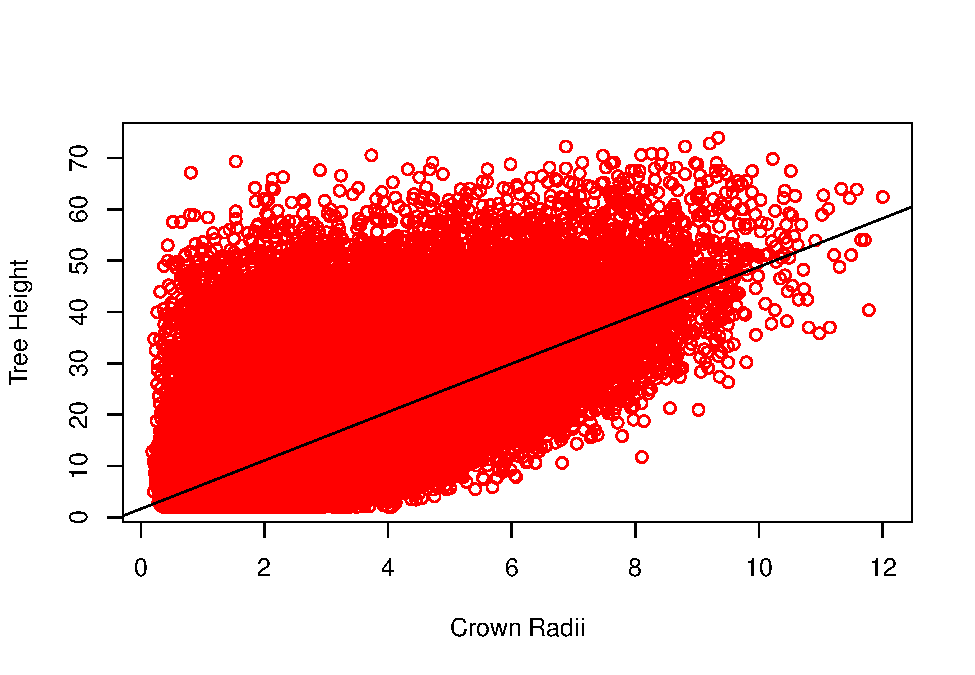
\includegraphics{BSmith_HW1_files/figure-latex/unnamed-chunk-5-1.pdf}

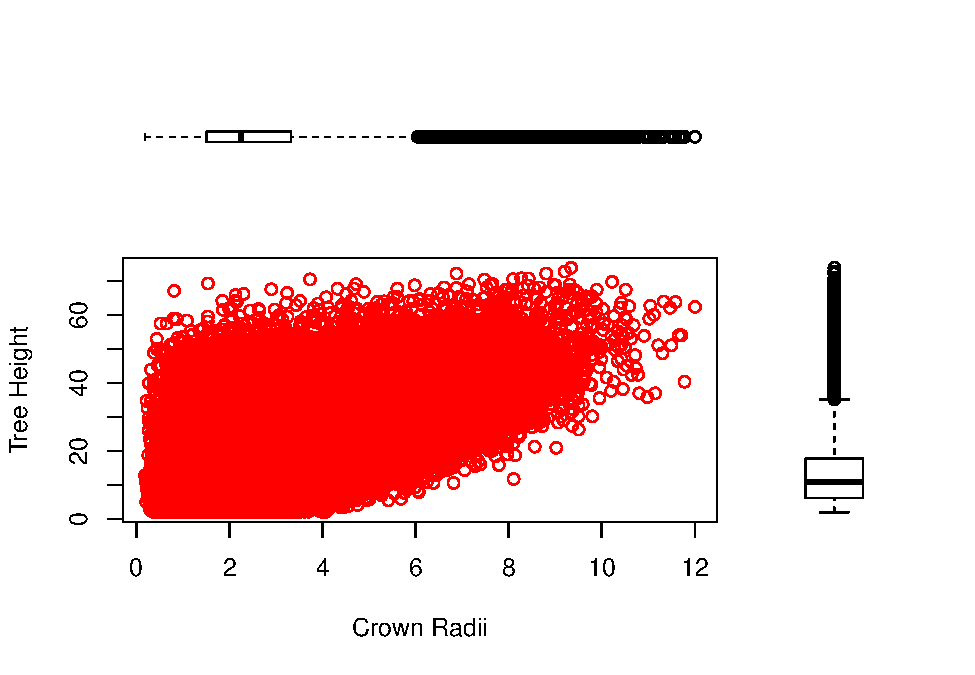
\includegraphics{BSmith_HW1_files/figure-latex/unnamed-chunk-6-1.pdf}

\textbf{Discussion:}

The uncorrected histograms indicate a left skewed distribution of tree
height and tree-crown radii. Once the values are corrected using a log
transformation, the histograms take on a normal distribution. This
analysis shows just how powerful data transformations can be when
analyzing data.

Plotting the tree height against the tree-crown radii with a scatterplot
offers good qualitative insight to the correlation between tree height
and tree-crown radii. Further analysis through the addition of a fitted
line shows that the data lies along the \texttt{x=y} line. The addition
of boxplots along the axes allows the viewer to visualize the
distribution of each dataset while simultaneously visualizing the
correlation.

The calculated Pearson's correlation coefficient, or r-value, is
0.6613456. This means that we have a strong positive correlation between
the tree-crown radii and height, which is to be expected. This also
confirms that we can reject the null hypothesis that there is no
correlation between tree-crown radii and height.

\textbf{Limitations:} The most notable limitations to RMarkdown is the
fact that you cannot underline or right-justify text. In terms of the
data, the crown density is not taken into account when performing this
analysis, and therefore could be considered an incomplete analysis.

\end{document}
